% Main document

\documentclass[english,12pt]{article}

% Für Deutsch
%\usepackage[utf8]{inputenc}
%\usepackage[ngerman]{babel}

% Packages
\usepackage{blindtext} % Lorem ipsum
\usepackage[a4paper,includeheadfoot,margin=2cm]{geometry} % Layout, showframe --> to see border
\usepackage{caption}
\usepackage[hidelinks]{hyperref} % links within the document and for clickable URLs
\usepackage{graphicx}
\usepackage[export]{adjustbox} % to beable to position images
\usepackage{amsmath} % equations
\usepackage{listings} % codeblocks
\usepackage{dirtytalk} % use quotations
\usepackage{titling} % So you can use theauthor
\usepackage[hybrid]{markdown} % Used to convert markdown

\usepackage[backend=bibtex,style=ieee]{biblatex} % or verbose-trad2

\bibliography{source.bib} % add sources to source.bib file

% Image
\graphicspath{{img/}}
\usepackage{float} % Allows putting an [H] (place HERE & not where LaTeX wants to put)

% Header & Footer
\usepackage{fancyhdr}

\usepackage{siunitx} % Required for alignment
\sisetup{
	round-mode          = places, % Rounds numbers
	round-precision     = 2, % to 2 places
}
\usepackage{booktabs} % For prettier tables

% Document information
\title{ZHAWo - Platform Independent Timetable App}
\author{Bachmann Dominik, Visser Julian}

% Header & Footer
\pagestyle{fancy}
\fancyhf{}
\lhead{PA - HS 2018}
\chead{}
\rhead{ZHAWo}
\lfoot{}
\cfoot{\thepage}
\rfoot{}

\begin{document}

	\setlength{\parindent}{0in} % removes default indent of new paragraph

	% !TEX root = pa_doc.tex

%----------------------------------------------------------------------------------------
%	TITLE PAGE
%----------------------------------------------------------------------------------------
\begin{titlepage} % Suppresses displaying the page number on the title page and the subsequent page counts as page 1
	\newcommand{\HRule}{\rule{\linewidth}{0.5mm}} % Defines a new command for horizontal lines, change thickness here

	\center % Centre everything on the page

	%------------------------------------------------
	%	Headings
	%------------------------------------------------

	
\includegraphics[width=0.3\textwidth, left]{./assets/zhawLogo.jpeg}\\[1cm]

	\textsc{\Large Projekt Arbeit}\\[0.5cm] % Major heading such as course name

	\textsc{\large HS 2018}\\[0.5cm] % Minor heading such as course title

	%------------------------------------------------
	%	Title
	%------------------------------------------------

	\HRule\\[0.5cm]

	%------------------------------------------------
	%	Logo
	%------------------------------------------------

	
\includegraphics[width=0.4\textwidth]{./assets/zhawoLogo.png}\\[0.5cm]

	\textsc{\large \textbf{ZHAWo} \\[0.2cm]
									--- \\[0.3cm]}
	% Title of your document
	\textsc{\large Platform Independent Timetable App}\\[0.5cm]


	\HRule\\[1cm]

	%------------------------------------------------
	%	Author(s)
	%------------------------------------------------

	\begin{minipage}{0.4\textwidth}
		\begin{flushleft}
			\large
			\textit{Authors}\\
			Bachmann Dominik \\
			Visser Julian % Your name
		\end{flushleft}
	\end{minipage}
	~
	\begin{minipage}{0.4\textwidth}
		\begin{flushright}
			\large
			\textit{Supervisor}\\
			Meier Andreas % Supervisor's name
		\end{flushright}
	\end{minipage}

	%----------------------------------------------------------------------------------------

	%------------------------------------------------
	%	Date
	%------------------------------------------------
	\vfill
	{\large\today} % Date, change the \today to a set date if you want to be precise

\end{titlepage}


	\pagenumbering{gobble}

	%Index
	\newpage
	\pagenumbering{roman}
	\tableofcontents
  \newpage
  \pagenumbering{arabic}

	% !TEX root = ba_doc.tex
\begin{abstract}
\begin{markdown}

\noindent Test
\noindent We also integrated news and events from the Verein Studierende ZHAW (vszhaw) into ZHAWo to provide students with easier access to information about events and services.

\noindent Using the JavaScript frameworks React for the frontend and Express for the backend in combination with Progressive Web App enables us to apply an agile development approach with fast prototyping of new features while still providing an application with the functionalities and feel that users expect from a native app. With this approach, we also avoid having to maintain multiple code bases for different platforms and mixing different technologies for frontend and backend. As a consequence, extending and improving the application's functionality can be done at a high velocity.

\end{markdown}
\end{abstract}

	\newpage

	% !TEX root = pa_doc.tex
\begin{markdown}

# Introduction

## Goals

Students of the Zurich University of Applied Sciences (ZHAW) have to visit multiple websites or use different applications on a daily basis in order to get information about their schedule, the offered menus in their campus mensa and events organized by the Verein Studierende ZHAW (vszhaw).

For their schedule, a student can either visit the official site \cite{Stundenplan} or use the official application for either Android \cite{AppAndroid} or iOS \cite{AppIOS}. The official site was designed for use on desktop browsers and is not optimised for responsiveness and display on phones. And while the official Android application is well maintained and offers a lot of additional features - such as direct access to public transport timetables and mensa menu plans - its iOS counterpart lacks many of these additional features and looks and feels rather unpolished in comparison. This difference in quality and features is a common occurrence because the development of native applications requires two separate code bases for Android and iOS. The most glaring issue with the iOS application is the lack of offline functionality. When a user's network cuts out, even the schedule information that was previously loaded can no longer be accessed after navigating away.

When students want to check the mensa menus of their campus, they have the option of visiting the SV groups site or to use the official Android or iOS application. These options suffer from the same issues as previously explained for the schedule.

With ZHAWo, our goal is to provide students with an improved application to have access to their schedule and mensa menus in one single cross-platform application. Additionally, with ZHAWo students can look for unoccupied rooms. This functionality was - until about two years ago - provided by an Android application that was no longer maintained and eventually disappeared from the Google Play Store. While the study rooms at, for example, the Technikum campus offer a space for both quiet work as well as group projects, in our experience as students it was very convenient to have a service to quickly look up free rooms without having to walk from room to room. Another feature ZHAWo provides is the integration of news and events of the vszhaw directly into the application. We aim to reduce the effort that is needed to stay up to date with the vszhaw and hope that both students and the vszhaw can profit from this.

By using Progressive Web Application (PWA) technologies \cite{PWA} in combination with JavaScript frameworks for both front- and backend, we achieve a consistent user experience on desktop, Android and iOS devices. We eliminate the issue of having to maintain separate code bases for different platforms while still being able to provide a native feel and functionality. PWA features such as offline caching of HTTP requests allow us to overcome previously mentioned issues with reliability on spotty networks.

An additional advantage we gain by using PWA technologies and the same programming language across the full stack is fast prototyping in an agile development process. Development of additional features and functionality can be achieved at a much faster rate with a single code base across all platforms.

\newpage

## Primary Functions

While our goal is to develop a feature rich application tailored to students of the ZHAW, we established the following four primary functions ZHAWo should provide in its prototype. Using an agile development approach, the scope of this project was to implement these primary functions in a prototype and adjust them to student feedback.

\begin{itemize}
  \item \textbf{Timetable}: A user can access their schedule and look up schedules of lecturers, classes, courses and rooms.
  \item \textbf{Menu plans}: A user can access menu plans of the different campus mensas across the ZHAW.
  \item \textbf{Room search}: A user can look for and find free rooms for a specific time-frame and location.
  \item \textbf{Student events}: A user can access vszhaw news and events to bring more attention to student parties and events.
\end{itemize}

After having established the core functionalities and a prototypical version of ZHAWo in the scope of this project, the features will be iteratively expanded and improved to end up with a production-ready application. For a full product backlog please refer to section 2.3.

\end{markdown}

  \newpage

  % !TEX root = pa_doc.tex
\begin{markdown}

# Development

## Agile Approach

For development of the ZHAWo prototype we used an iterative agile approach. The code base was managed on a single GitHub repository \cite{DUMMY} for both front- and backend. User stories were tracked using GitHub issues and the sprints were organized using GitHub project boards. Over the course of the project, we structured the development into six sprints of 2 weeks. We regularly considered feedback of other students and our own review of our practices and used technologies in our planning. The flexibility of using only JavaScript and PWA technologies enabled us to rapidly prototype new ideas without the hassle of having to maintain two different code bases.
User stories were implemented and tested in feature branches and merged into the master branch as part of the sprint reviews. This practice ensured that we had - for the most part - stable new iterations of the application to deploy for user feedback.

## Continuous Integration \& Deployment

For continuous integration we used Travis CI \cite{DUMMY} in combination with Codecov \cite{DUMMY} to track test coverage. With good integration of both these tools into GitHub - for example reporting of build status and test coverage changes in GitHub comments on each pull request - we achieved good code and test quality across feature implemenations and sprints.
While the goal is to eventually host our application on a ZHAW server, in the scope of this project the prototype was deployed to Heroku \cite{DUMMY} and shared amongst students for quick feedback on new features.

\newpage

## Product Backlog

The following planned user stories have been implementat in the scope of this project. We put the focus on implementing the schedule context of ZHAWo in detail and provide prototypical functionality for the other primary functionalites. For implementation details please refer to section 3.

\begin{itemize}
  \item \textbf{US01}: As a user I want to save my credentials/username
  \item \textbf{US02}: As a user I want the app to work even when I don't have network connection
  \item \textbf{US03}: As a user I want to switch between contexts (schedule, menus, room search, vszhaw)
  \item \textbf{US10}: As a user I want to view my timetable/schedule for a day
  \item \textbf{US11}: As a user I want to vew my timetable for a week
  \item \textbf{US12}: As a user I want to navigate to the current day
  \item \textbf{US13}: As a user I want to navigate between days when using the day view (timetable)
  \item \textbf{US14}: As a user I want to navigate between weeks (timetable)
  \item \textbf{US15}: As a user I want to navigate to a specific date in a month view (timetable)
  \item \textbf{US16}: As a user I want to view a specific rooms timetable
  \item \textbf{US17}: As a user I want to view a specific classes timetable
  \item \textbf{US18}: As a user I want to view a specific courses timetable
  \item \textbf{US19}: As a user I want to view a specific persons timetable
  \item \textbf{US20}: As a user I want to have a detailed view of my events
  \item \textbf{US30}: As a user I want to find currently unoccupied rooms
  \item \textbf{US56}: As a user I want to see prices for all menus
  \item \textbf{US58}: As a user I want to view a specific mensas menu plan
  \item \textbf{US70}: As a user I want to view vszhaw blog posts/event announcements
\end{itemize}

\newpage

The following user stories are planned to be implemented in the finished application. This list will of course be extended and adjusted based on user feedback and our own review.

\begin{itemize}
  \item \textbf{US31}: As a user I want an overview of my campus with highlighted buildings where there are unoccupied rooms
  \item \textbf{US32}: As a user I want a floor plan of each floor per building with highlighted unoccupied rooms
  \item \textbf{US33}: As a user I want to navigate between buildings through the overview of my campus
  \item \textbf{US34}: As a user I want to navigate between floor plans of a building
  \item \textbf{US35}: As a user I want to see until when a room is unoccupied
  \item \textbf{US36}: As a user I want to filter my search to only show rooms that are unoccupied for at least x hours/minutes
  \item \textbf{US50}: As a user I want to view the mensa menu for my campus for a day
  \item \textbf{US51}: As a user I want to view the mensa menu for my campus for a week
  \item \textbf{US52}: As a user I want to navigate to the mensa menu of the current day
  \item \textbf{US53}: As a user I want to navigate between days when using the mensa menu day view
  \item \textbf{US54}: As a user I want to navigate between weeks when using the mensa menu week view
  \item \textbf{US55}: As a user I want to navigate to a specific date in a month view (mensa menu)
  \item \textbf{US57}: As a user I want to navigate between menus of different days
\end{itemize}

\end{markdown}

  \newpage

	% !TEX root = pa_doc.tex
\begin{markdown}

# Implementation

## Frontend
For the presentation of the web application to the user, we used React\cite{React}. We decided to use React because of its potential to write cleaner code with component based modularity. To minimise potential problems and to insure a a unidirectional data flow we chose to incorporate  the flux pattern into the architecture design, instead of using the typical Model View Controller (MVC) architecture.

The data for the front end is provided by the back end RESTful API service and retrievable through HTTP calls. Each fetch request is cached using a service worker. We built the service worker using Workbox\cite{Workbox}. Workbox is a library that implements in a set of service worker best practices and helps you get the most out of your service workers.

### PWA
\say{Progressive Web Apps (PWA) are experiences that combine the best of the web and the best of apps.}\cite{WhatIsPWA}

Google and other companies have developed a new, modern web application standard. PWAs implement said standard and receive additional permission as a rewarded for doing so. This allows PWA to behave and feel like native apps. They live can on the user's home screen, offer a full screen experience, access device hardware (camera, GPS, etc) and can even re-engage users with push notifications\cite{PWA}.  When launched from the user’s home screen a Progressive Web App can load instantly, regardless of the network state. This is done by with the help of service workers.

#### Service Workers
A service worker is like a client-side proxy and that allows control of the cache. You can improve the loading speed of your page by pre-caching key resources. Using cache also eliminates the dependence on the network, ensuring a reliable offline experience for your users.\cite{ServiceWorker}

### React
React\cite{React} was originaly developed by Facebook and is one of the most popular UI librarys. It allows you to create reusable Compents using JSX, a syntax extension to JavaScript.
The idea behind React is to design simple views for each state of the application. Doing so allows it to only update and render components that need to be changed, thereby improving performance immensely.

#### Flux
Flux\cite{OurReadme} is a application pattern developed by Facebook. It's goal is to insure a a unidirectional data flow in React apps. The use of this practice enhances the quality and performance of the code by improving the data consistency. It is the optimal architecture for the use of React.

\begin{figure}[H]
  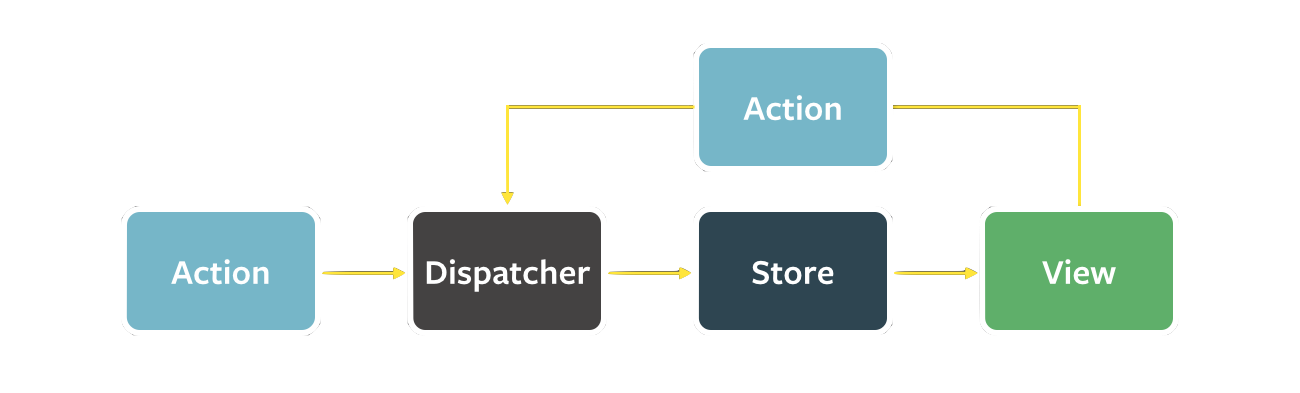
\includegraphics[width=10cm, center]{./assets/flux.png}
  \caption{Flux Model{\cite{FluxModel}}}
\end{figure}



% TODO: bild ref https://facebook.github.io/flux/img/flux-simple-f8-diagram-with-client-action-1300w.png

In Flux, the dispatcher is a singleton that directs the flow of data to ensure that updates do not cascade, which would lead to unpredictable behaviour. When a user interacts with a React view, the view sends an action through the dispatcher, which notifies the stores that hold the application’s data. When the stores change state, the view gets notified and changes accordingly.


## Backend
The Sever-side of ZHAWo is implemented in NodeJS\cite{Node}. We use the ExpressJS Server to handle all the API calls.

### NodeJS
Node.js is a JavaScript runtime environment, designed to build scalable network applications\cite{Node}.
*öpis vo da https://nodejs.org/en/about/* blocking and so on
#### Express
Express\cite{Express} is a minimal and flexible web application framework for Node.js. It provides HTTP utility methods and allows you to create a robust API.

% TODO: add image front-back api calls and stuff

% TODO: expand this, explain CampusInfo -> why we needed our own backend blabla

\end{markdown}

  \newpage

  % !TEX root = pa_doc.tex
\begin{markdown}

# Discussion

We were able to implement a prototype of ZHAWo as a Progressive Web App which covers all primary functions that were planned. Students can access their schedule, mensa plans and the news and event feed from vszhaw. Additionally, they can get a list of free rooms that can then be used as a distraction free work space. We were able to share the prototype with a small group of students and user feedback for our application was positive.

Using a full JavaScript technology stack for front- and backend and Progressive Web Apps has proven to work well with an agile development approach. While developing native applications, having to maintain different code bases can be awkward in combination with agile principles. The strength of the agile development approach that we have chosen is that we can prototype new features rapidly and can receive user feedback from both Android and iOS users immediately. In addition to that, not having to stay up to date with best practices, libraries and frameworks for different languages such as Java/Kotlin and Swift/Objective C for Android and iOS development respectively allowed us to implement new features at a faster pace.

While there are obvious advantages to building ZHAWo as a cross platform PWA, we have also identified some weaknesses. Installing an application not through the App Store or the Google Play Store is unexpected for most users. There are also some inconsistencies in support offered by different platforms. We attribute most of our issues to PWA technologies being relatively new and expect both support and users familiarity with the concept of PWAs to increase in the near future.

In a second part of this project, we aim to improve the user experience further and extend ZHAWo with more features.

\end{markdown}

  \newpage

	%\markdownInput{example.md}

	\section{Appendix}

	\listoffigures
  % \listoftables

	%\renewcommand\refname{Literaturverzeichnis} % rename --- für Deutsch
	\printbibliography % Uses source.bib to make ref table

\end{document}
